\chapter{Introduction}
\label{cp:introduction}
The University of Moratuwa is situated in close proximity to the Bolgoda Environmental Protection Area (EPA). Additionally, within the university grounds lies a natural terrestrial ecosystem commonly referred to as 'Kaju Kele.' This unique setting has established the University of Moratuwa as one of the urban universities in Sri Lanka with the highest diversity of bird species.
\\\\
The last study conducted on the bird diversity at the University of Moratuwa dates back almost 10 years, utilizing data collected from August 2003 to March 2005[1]. The present paper is based on more recent data, spanning from October 2021 to January 2024, collected by the two authors.
\\\\
The first volume of this series focuses on bird diversity, and upcoming volumes may explore other classes of flora \& fauna.
\begin{figure}[!htpb]
    \centering
    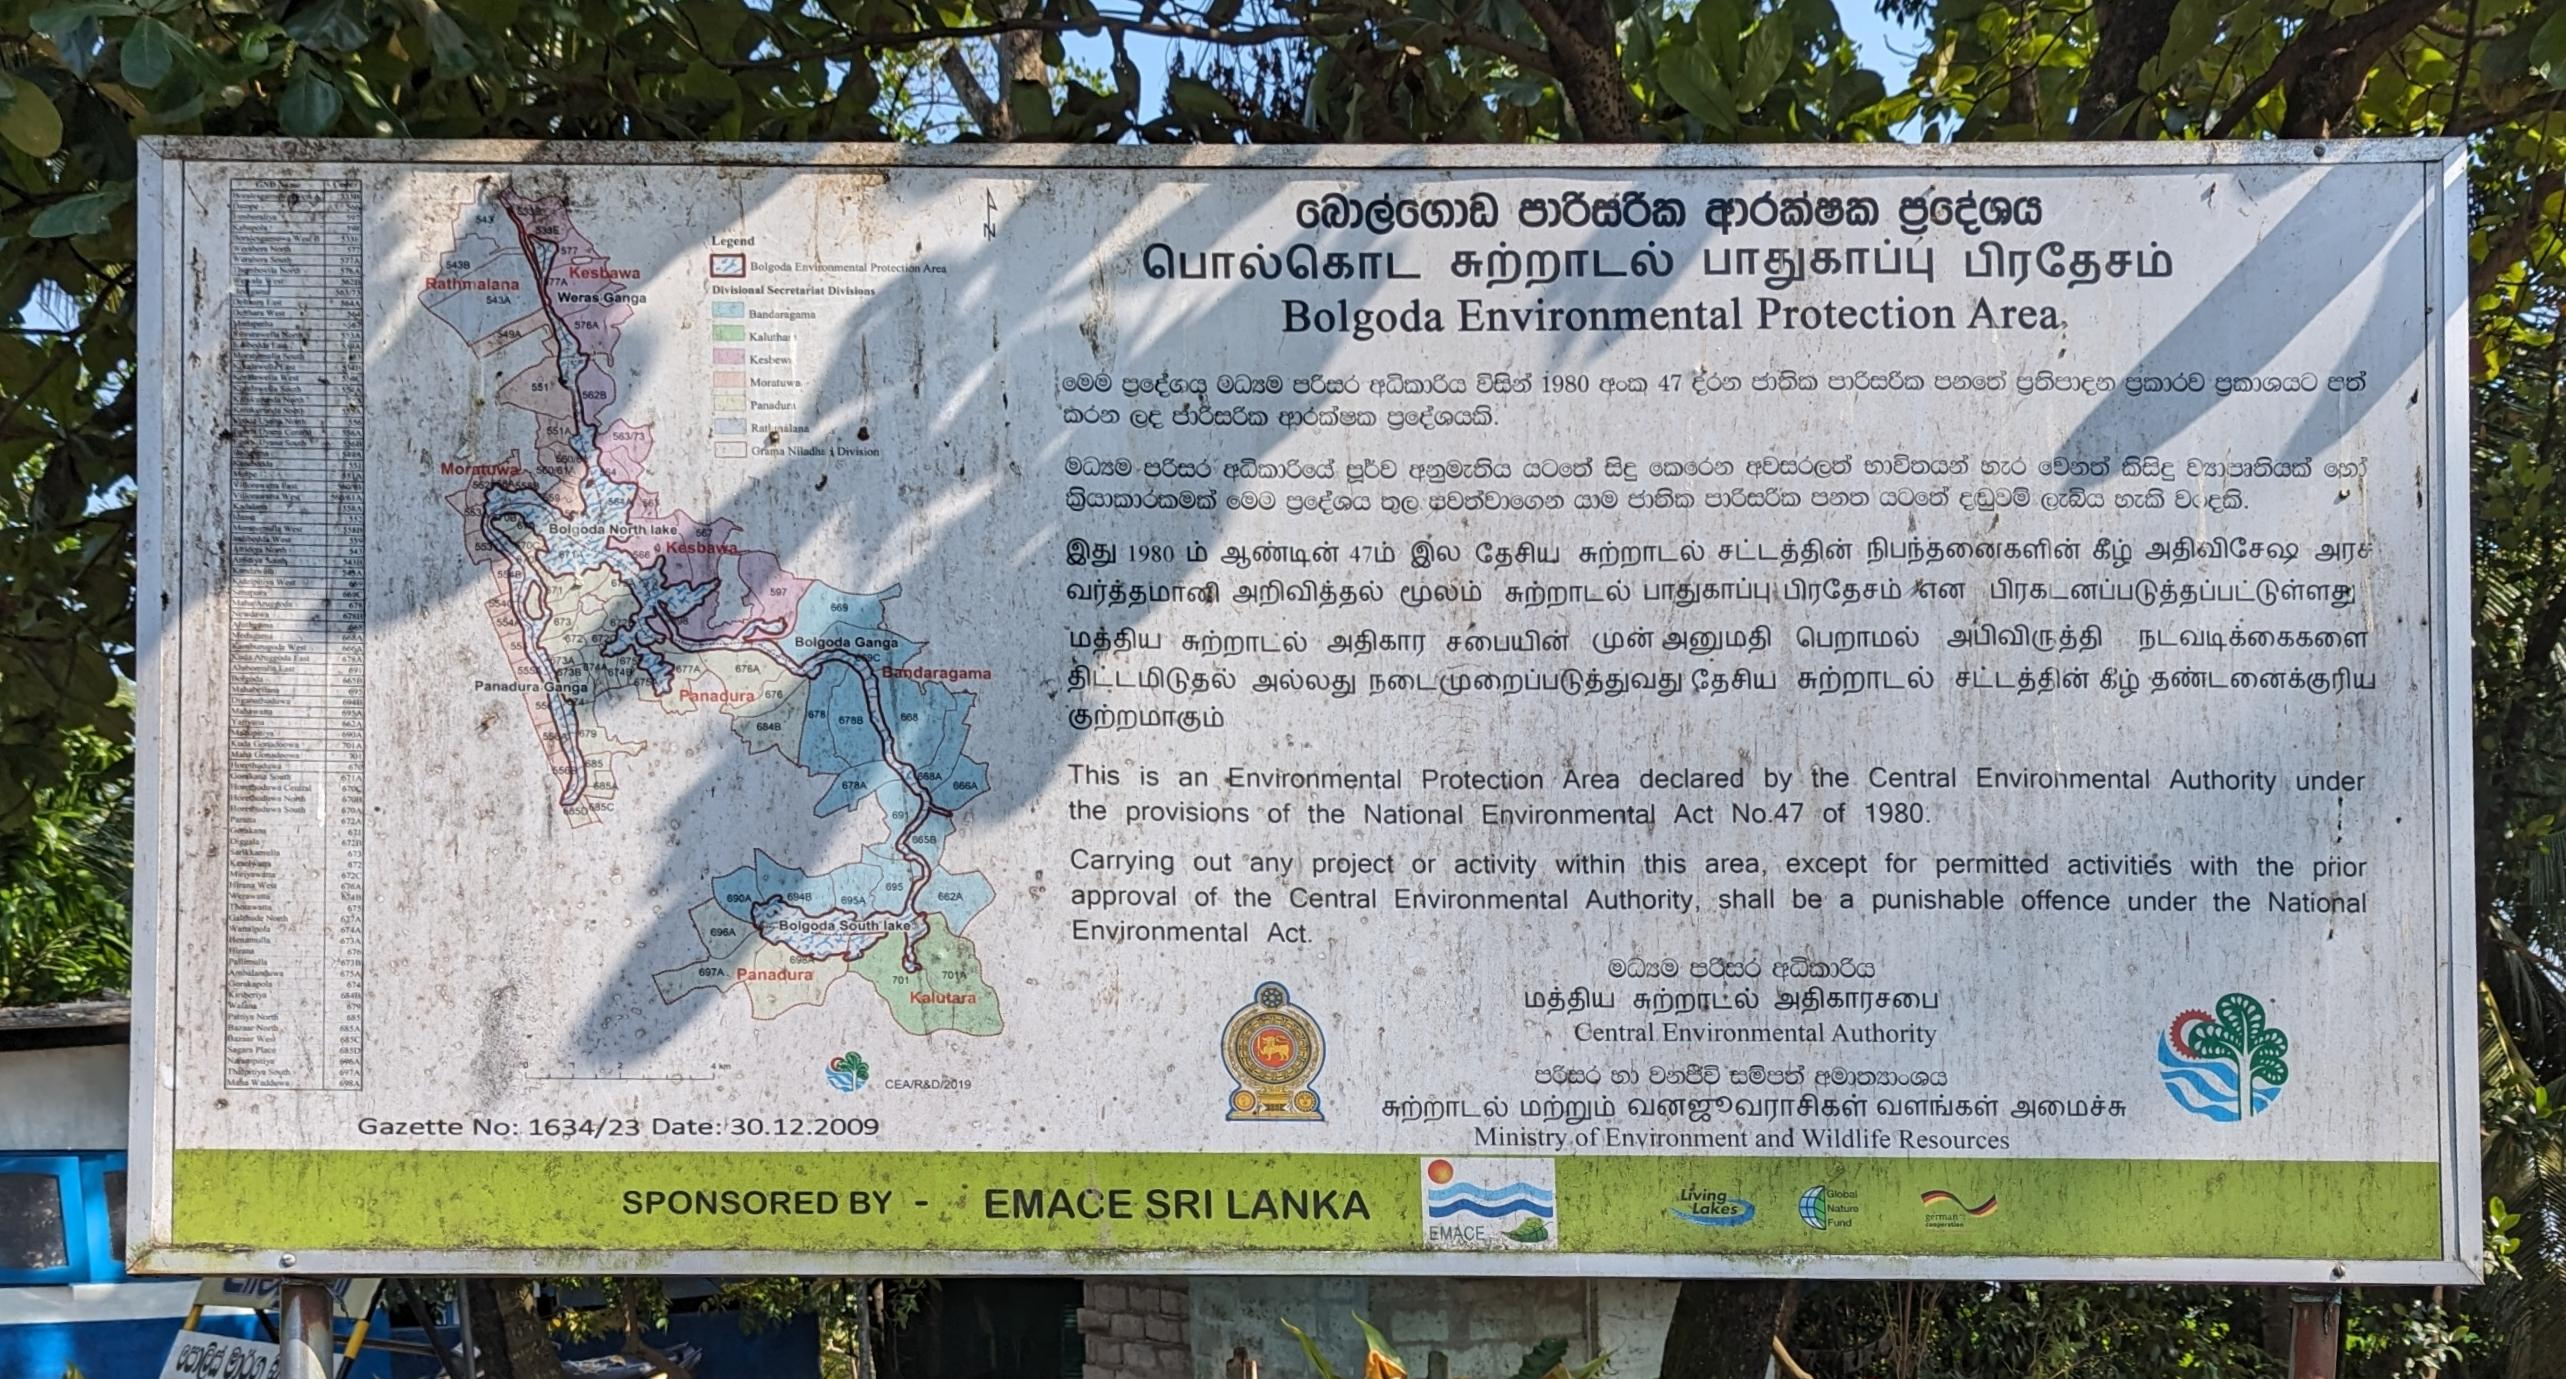
\includegraphics[width=0.9\textwidth]{Figures/epa.jpg}
    \caption[]{The Bolgoda EPA.}
    \label{fig:figure-01}
\end{figure}

% \nameref{cp:citations} (referred to as \autoref{cp:citations}).